\section{Модель диффузии мономера в слое ПММА}

Оценка времени диффузии мономера, образующегося в слое ПММА в процессе СЭЛТР, проводилась на основе значений коэффициента диффузии, приведенных в работе~\cite{Karlsson2001_diffusion} (среднечисловая молекулярная масса ПММА в этой работе составляла 30000 г/моль). Для получения оценки для времени диффузии сверху была рассмотрена минимальная из температур -- 135~$^\circ$C.
Значение коэффициента диффузии ММА в ПММА при 135~$^\circ$C (2\:$\cdot$\,10$^\text{-10}$ см$\pp$/с) было пересчитано для резиста PMMA 950K A2 со среднечисловой молекулярной массой около 271000~г/моль, использовавшегося в данной работе, на основе формулы~\ref{eq:diffusion_Mn}:
\begin{equation}
	\begin{cases}
		\lg D_{30000} = \lg D_{\infty} + \displaystyle{\frac{k}{30000}}, \vspace{0.4em} \\
		\lg D_{271000} = \lg D_{\infty} + \displaystyle{\frac{k}{270000}},
	\end{cases}
\end{equation}
где $k$ = 1.06\:$\cdot$\,10$^\text{4}$. Это приводит к следующему выражению для коэффициента диффузии ММА в ПММА при 135~$^\circ$C (в см$\pp$/с):
\begin{equation}
	D_{271000}^{135 \, ^\circ \mathrm{C}} = D_{30000} \cdot 10^{k \left(\frac{1}{271000} - \frac{1}{30000} \right)} = 2 \cdot 10^{-10} \cdot 10^{1.06 \cdot 10^4 \left(\frac{1}{271000} - \frac{1}{30000} \right)} \cong 9.7 \cdot 10^{-11}.
\end{equation}
При экспонировании локальная молекулярная масса ПММА уменьшается, что приводит к увеличению коэффициента диффузии. Согласно формуле~\ref{eq:diffusion_Mn}, коэффициент диффузии ММА в ПММА (в см$\pp$/с) для ПММА со среднечисловой молекулярной массой $M_\mathrm{n}$ < 271000 при температуре 135~$^\circ$C может быть рассчитан по формуле
\begin{equation} \label{eq:D_Mn}
	D_{\Mn}^{135 \, ^\circ \mathrm{C}} = 9.7 \cdot 10^{-11} \cdot 10^{1.06 \cdot 10^4 \left( \frac{1}{271000} - \frac{1}{\Mn} \right)}.
\end{equation}
Данная зависимость приведена на рисунке~\ref{fig:Mn_diff}.

Для оценки времени выхода мономера из слоя ПММА проводилось численное решение уравнения диффузии для мономера, образовавшегося в слое ПММА за 1~секунду экспонирования. Начальное распределение количества свободного мономера в слое ПММА получалось за счет умножения промоделированного распределения числа разрывов молекул ПММА, произошедших за 1~секунду экспонирования, на среднюю длину кинетической цепи при деполимеризации (принятую равной 500 для температуры 135~$^\circ$C). Далее время выхода мономера из слоя ПММА оценивалось как время, за которое концентрация мономера в центре линии уменьшается в 10 раз.
При исходном коэффициенте диффузии (9.7\:$\cdot$\,10$^\text{-11}$~см$\pp$/c) это время составляет около 15 с (рисунок~\ref{fig:diffusion_initial}). Однако, уже после 10 секунд экспонирования среднечисловая молекулярная масса резиста на краях линии снижается до $\cong$1\:$\cdot$\,10$^\text{4}$ г/моль, что соответствует значению коэффициента диффузии около 1\:$\cdot$\,10$^\text{-9}$ см$\pp$/c. В этом случае время, за которое концентрация мономера в центре линии уменьшается в 10 раз составляет около 1 с (рисунок~\ref{fig:diffusion_10s}).

\begin{figure}[h]
	\begin{center}
		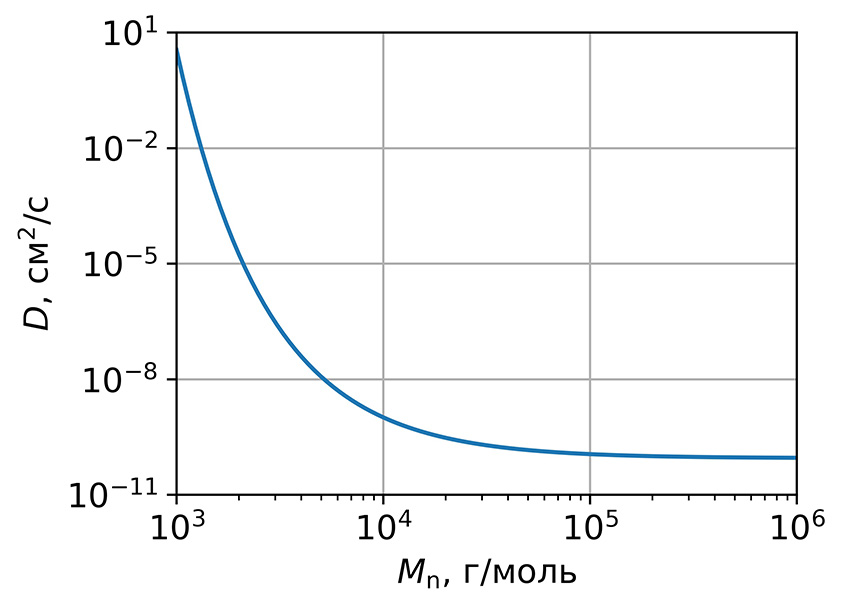
\includegraphics[width=0.6\linewidth]{diffusion/DD_12_straight_200}
	\end{center}
	\vspace{-1em}
	\caption{Зависимость коэффициента диффузии ММА в ПММА ($D$) от среднечисловой молекулярной массы ПММА ($\Mn$) при 135~$^\circ$C.}
	\label{fig:Mn_diff}
\end{figure}

Учитывая то, что в вышеописанных вычислениях использовался коэффициент диффузии на краях линии, в центре линии (где молекулярная масса резиста в разы меньше (рисунок~\ref{fig:Mn_hist}) значение коэффициента диффузии будет в разы выше согласно формуле~\ref{eq:D_Mn}. Принимая также во внимание тот факт, что данные расчеты относятся к минимальной из температур, при которых проводились эксперименты по исследованию метода СЭЛТР, можно заключить, что по сравнению с характерным временем экспонирования временем диффузии мономера из слоя ПММА в процессе СЭЛТР можно пренебречь. Это также подтверждает предположения о быстрой диффузии мономера, сделанные в работе~\cite{Bruk_2013} на основе формулы для времени диффузионного проскока молекул газа через слой толщины $l$:
\begin{equation} \label{eq:Bruk_tau_diff}
	\tau_{\text{diff}} = \frac{l^2}{12 D_\mathrm{e}},
\end{equation}
где $D_\mathrm{e}$ -- эффективный коэффициент диффузии газа. При толщине слоя 500 нм и значении коэффициента диффузии 9.7\:$\cdot$\,10$^\text{-11}$ см$\pp$/с время $\tau_{\text{diff}}$, вычисленное по формуле~\ref{eq:Bruk_tau_diff} составляет около 2 с.

В силу полученных оценок для времени диффузии мономера из слоя \linebreak ПММА в дальнейшем будет считаться, что весь образующийся мономер мгновенно покидает слой ПММА.

\begin{figure}[H]
	\begin{center}
		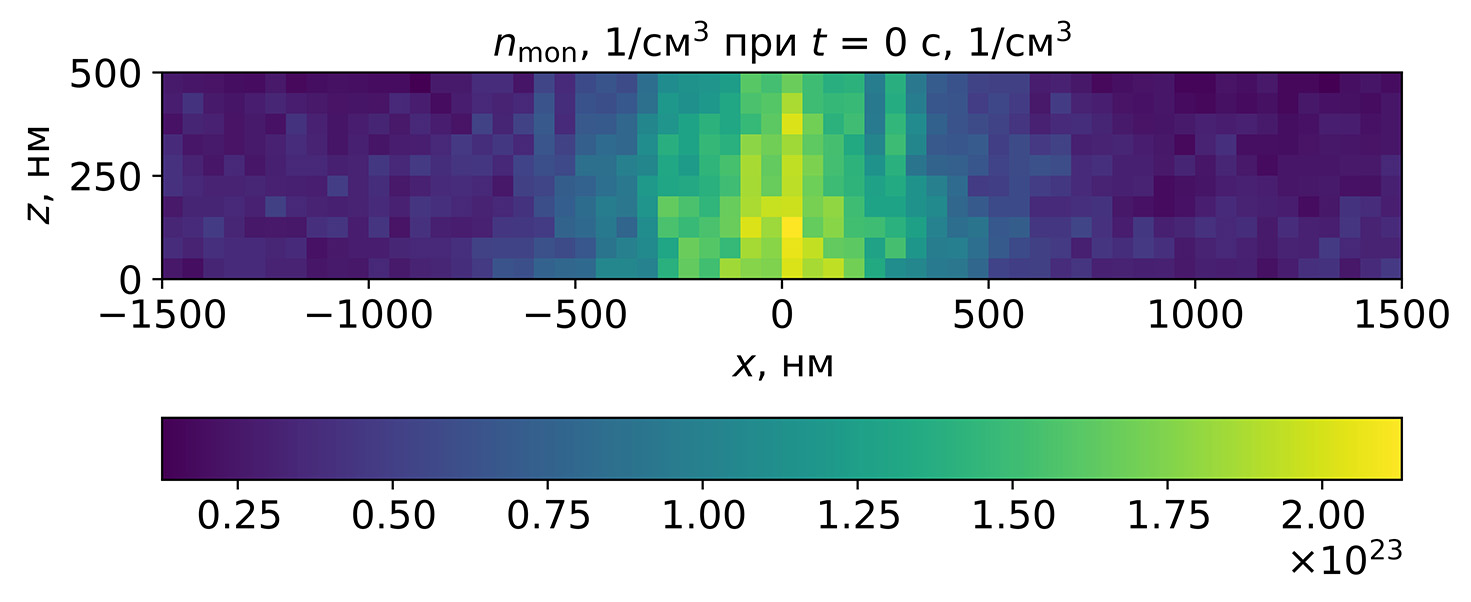
\includegraphics[width=0.8\linewidth]{diffusion/n_mon_initial_straight_200} \\
		\vspace{-4em} \text{\hspace{-26em} a)} \vspace{2.2em} \\
		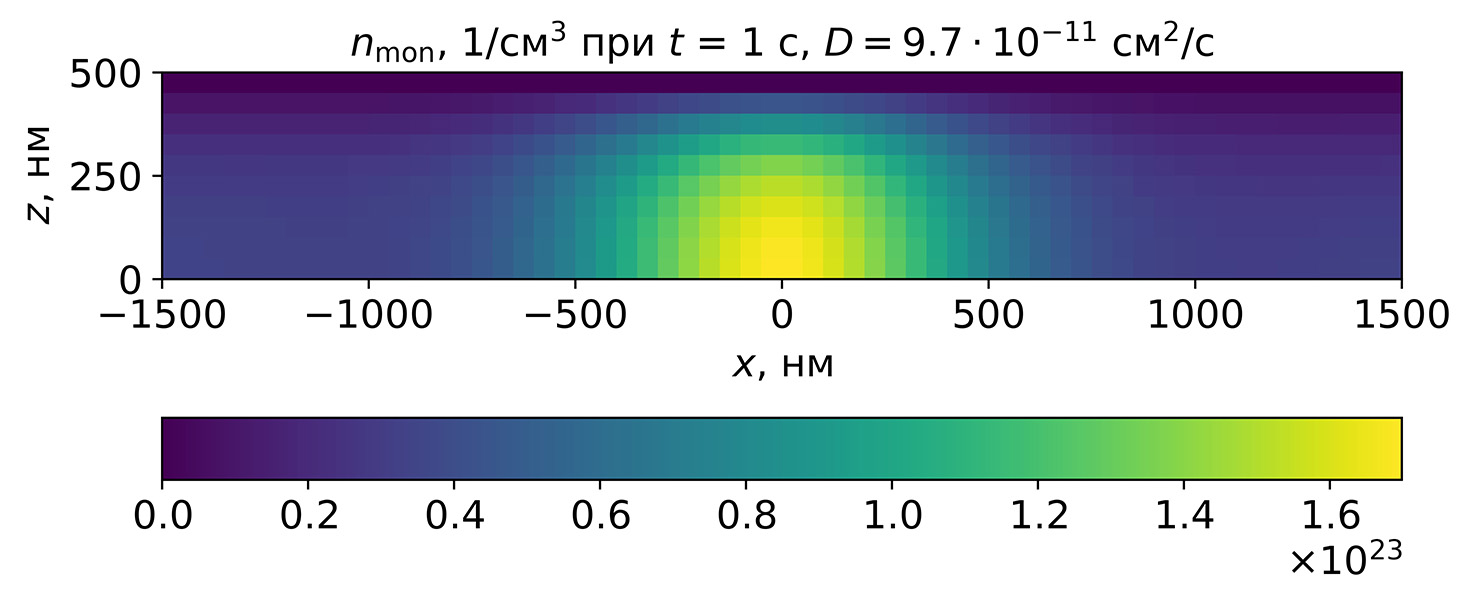
\includegraphics[width=0.8\linewidth]{diffusion/n_mon_9p7e-11_1s_straight_200} \\
		\vspace{-4em} \text{\hspace{-26em} б)} \vspace{2.2em} \\
		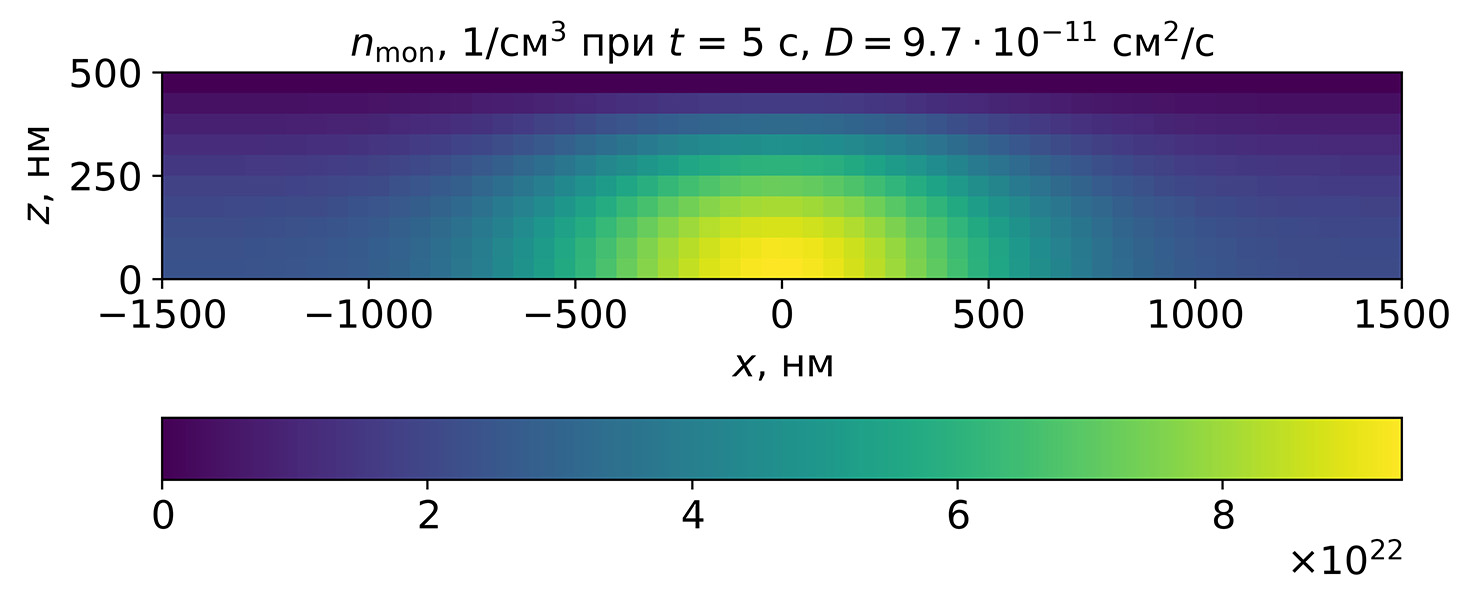
\includegraphics[width=0.8\linewidth]{diffusion/n_mon_9p7e-11_5s_straight_200} \\
		\vspace{-4em} \text{\hspace{-26em} в)} \vspace{2.2em} \\
		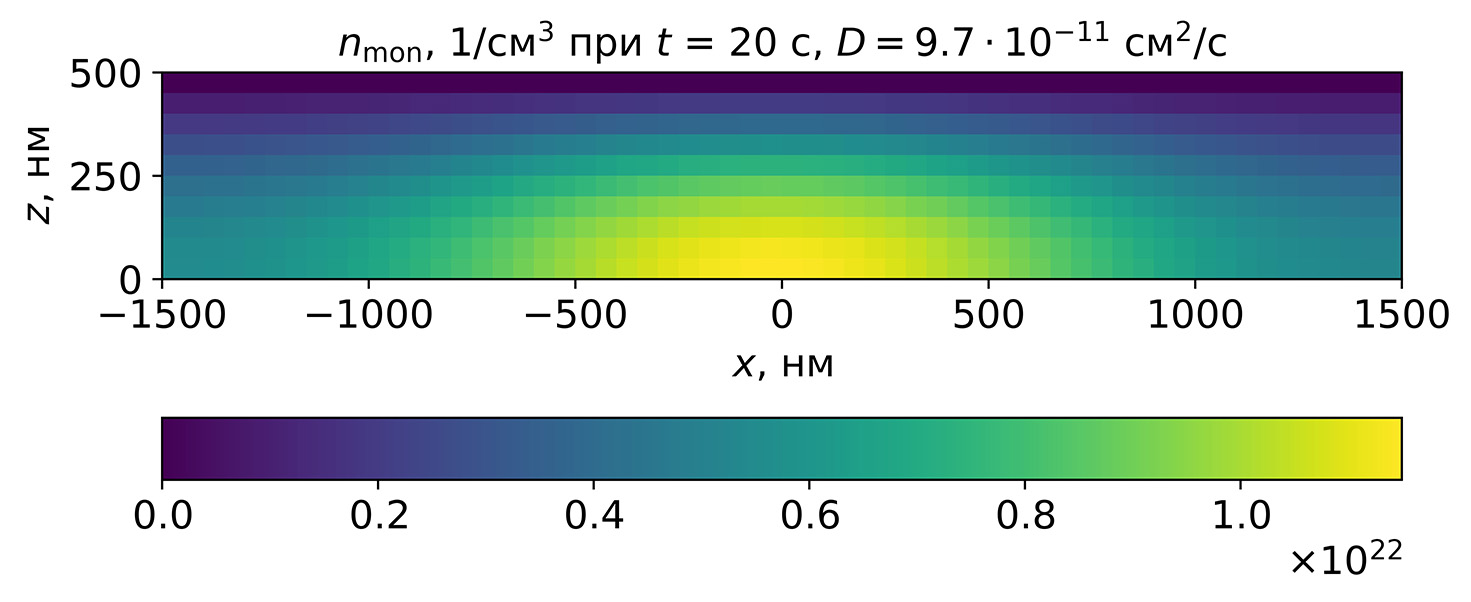
\includegraphics[width=0.8\linewidth]{diffusion/n_mon_9p7e-11_20s_straight_200} \\
		\vspace{-4em} \text{\hspace{-26em} г)} \vspace{2.2em} \\
	\end{center}
	\vspace{-1em}
	\caption{Распределение концентрации мономера, выделившегося в слое ПММА за 1 с экспонирования при температуре 130~$^\circ$C, в различные моменты времени. Коэффициент диффузии ММА в ПММА равен 9.7\:$\cdot$\,10$^\text{-11}$ см$\pp$/c.}
	\label{fig:diffusion_initial}
\end{figure}

\newpage

\begin{figure}[H]
	\begin{center}
		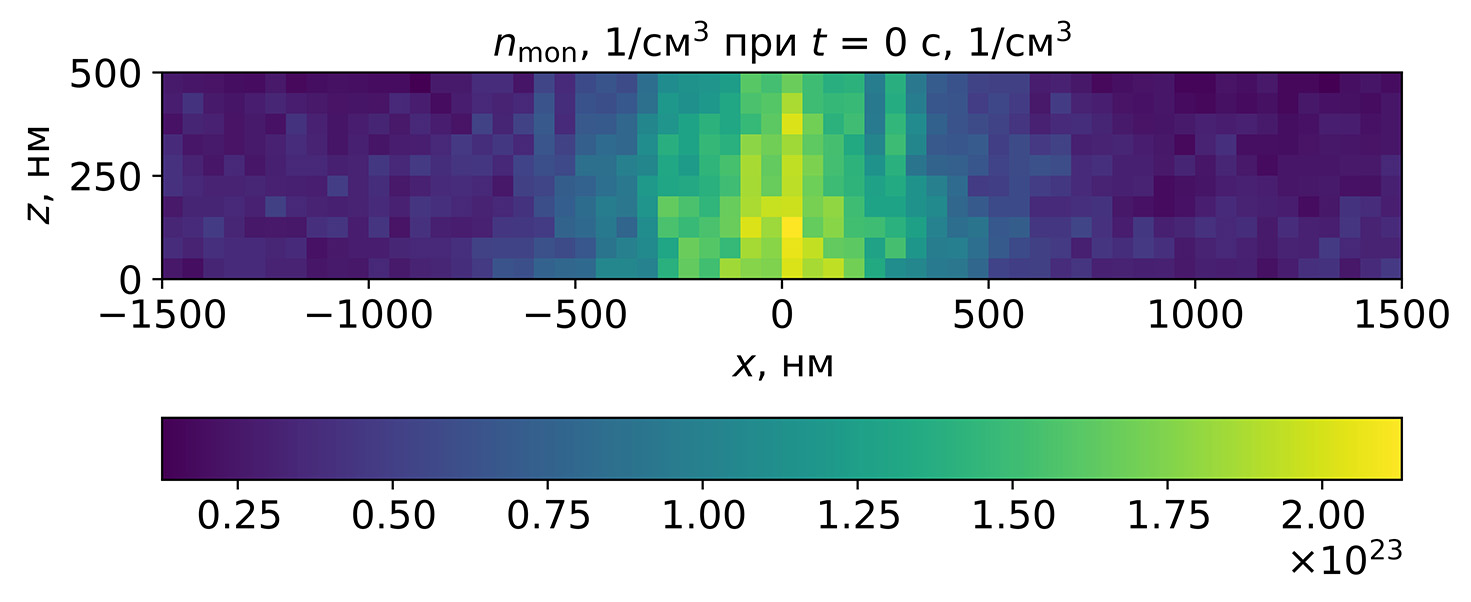
\includegraphics[width=0.8\linewidth]{diffusion/n_mon_initial_straight_200} \\
		\vspace{-4em} \text{\hspace{-26em} a)} \vspace{2.2em} \\
		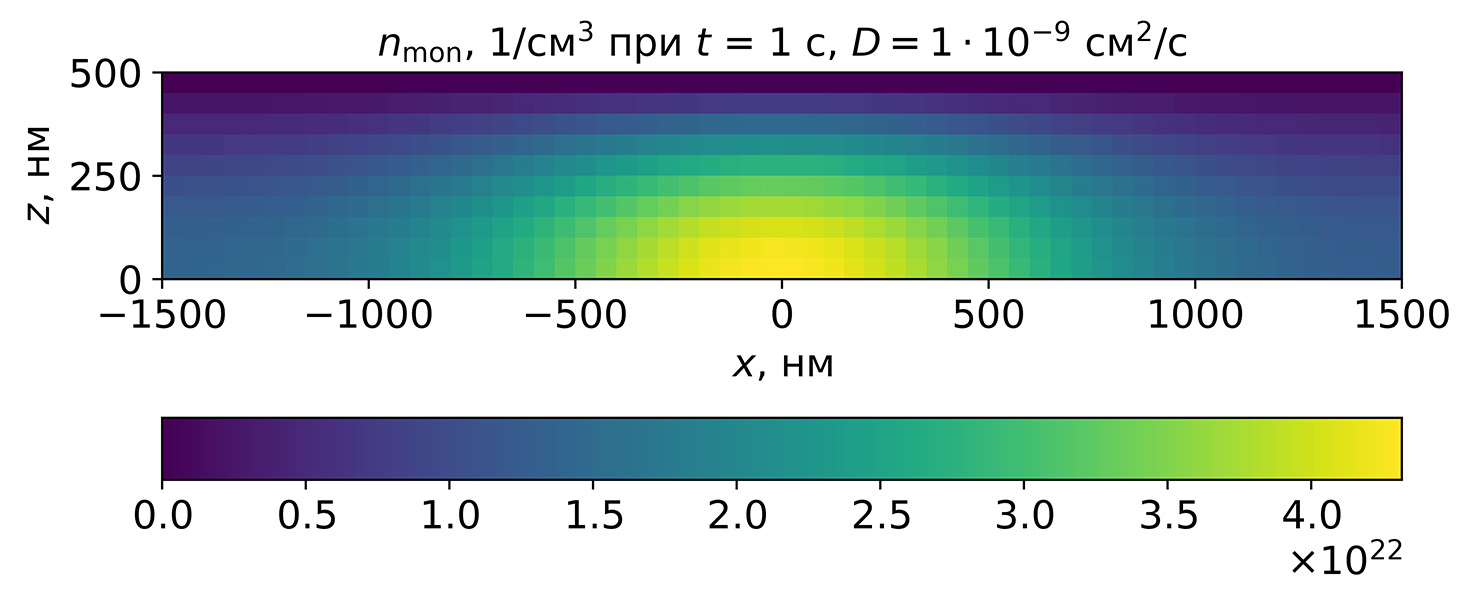
\includegraphics[width=0.8\linewidth]{diffusion/n_mon_1e-9_1s_straight_200} \\
		\vspace{-4em} \text{\hspace{-26em} б)} \vspace{2.2em} \\
		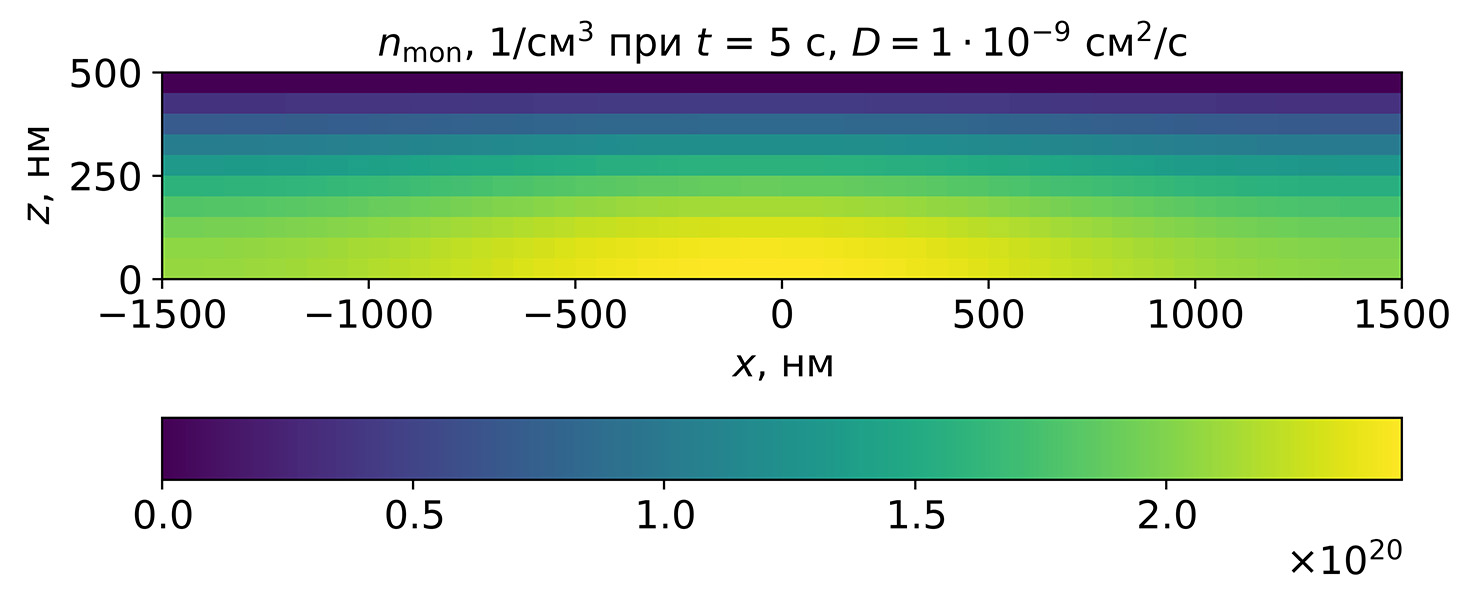
\includegraphics[width=0.8\linewidth]{diffusion/n_mon_1e-9_5s_straight_200} \\
		\vspace{-4em} \text{\hspace{-26em} в)} \vspace{2.2em} \\
		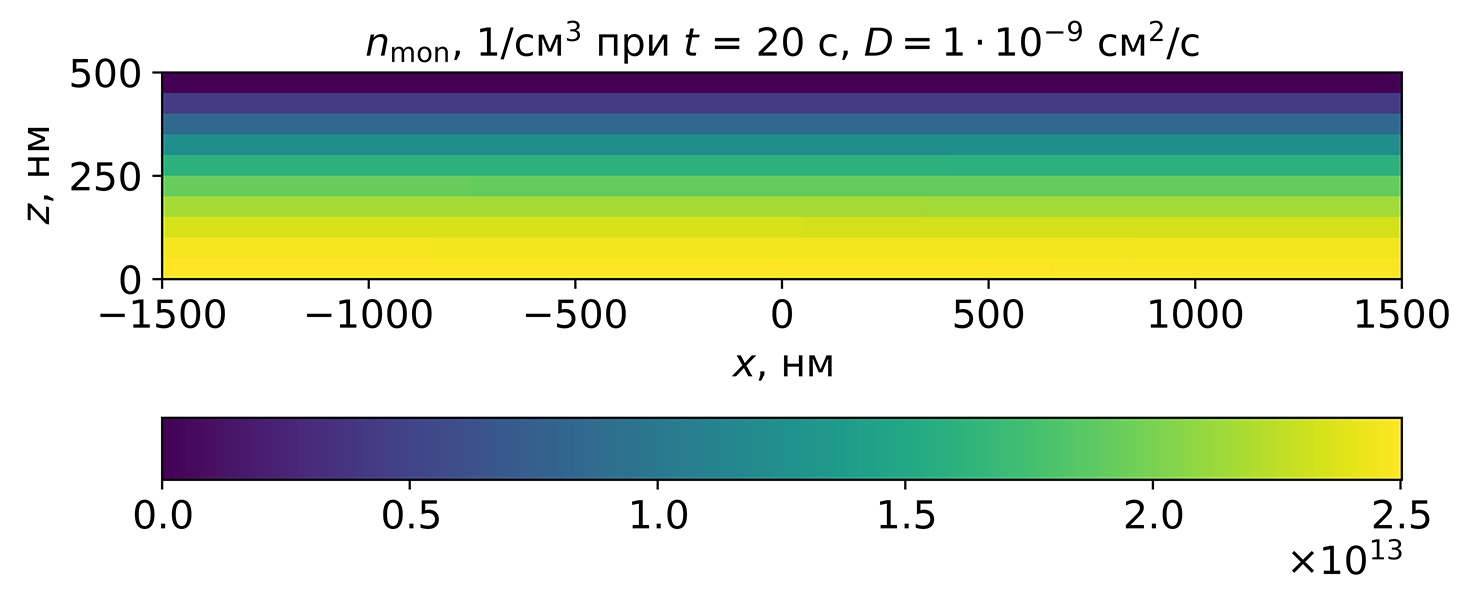
\includegraphics[width=0.8\linewidth]{diffusion/n_mon_1e-9_20s_straight_200} \\
		\vspace{-4em} \text{\hspace{-26em} г)} \vspace{2.2em} \\
	\end{center}
	\vspace{-1em}
	\caption{Распределение концентрации мономера, выделившегося в слое ПММА за 1 с экспонирования при температуре 130~$^\circ$C, в различные моменты времени. Коэффициент диффузии ММА в ПММА равен 1\:$\cdot$\,10$^\text{-9}$ см$\pp$/c.}
	\label{fig:diffusion_10s}
\end{figure}
